\chapter{二维硼化钛的高通量结构搜索和超导性质研究}
% for Roman nomber font
\newcommand*{\rom}[1]{\uppercase\expandafter{\romannumeral #1\relax}}

硼元素因为具有独特的多中心键,其化合物在低维时能够展现出丰富的结构多样性。现在已经被实验发现的,就包括许多的零维硼团簇和二维硼平面。在稳定的硼团簇中,\ce{B12}\cite{kiran2009origin}是最为稳定的结构之一,它可以被看作是平面三角网格的零维碎片。当原子数持续增加,硼平面团簇的结构中会出现空位,这样六边形空位的出现使得团簇更稳定。在\ce{B30}和\ce{B36}\cite{pham2014boron}中都存在这样的空位,而这样具有空位的结构是该原子数的硼团簇中最为稳定的。

过渡到二维硼平面,为了平面结构在能量上更加稳定,同样需要在结构中出现如团簇平面中的六角形空位。在已经被理论计算预言的稳定的硼单层平面中,$\alpha$-硼平面\cite{yang2008ab}的单胞中就有硼六角空位。根据该结构规律,我们课题组先前的工作中\cite{xu2017practical},给出了一系列具有相似结构特征的稳定硼平面结构,并总结了硼平面结构稳定的结构规律与化学原因。此外,其他课题组还发现了许多硼平面结构的新奇物理化学性质,如超导性质\cite{penev2016can,zhao2016superconductivity},拓扑性质\cite{feng2017dirac},二维硼半导体\cite{xu2017two}等。

通过在硼平面或硼团簇中嵌入金属元素,尤其是过渡金属元素,硼元素化合物的结构多样性会变得更加的丰富,也因此能够表现出更为丰富的性质。比如,准单层的\ce{TiB2}结构的能带中可以观察到狄拉克锥\cite{zhang2014prediction},其费米能级处的电子迁移率能够和石墨烯媲美。二维的\ce{MoB4}\cite{xie2014first}则在费米能级处有双狄拉克锥,同样有极好的电子迁移率。实验上,已经发现了许多过渡金属与硼构成的稳定多配位平面团簇结构\ce{TM}@\ce{B_n}。我们认为,这些过渡金属硼平面团簇结构,可以看作是过渡金属硼平面的结构碎片,从而充当构成稳定过渡金属硼平面的构筑单元。
相似的已经报导的过渡金属硼化物还包括,理论计算预测第四周期过渡金属硼平面中,\ce{FeB6}\cite{li2016global}为半导体,\ce{CrB4}\cite{li2019room}为单层铁磁材料并有高达\SI{401}{\kelvin}的居里温度。

而过渡金属因其未配对的$d$轨道电子,还会展现出丰富的磁学和电学性质。
超导性质作为一种有重要实用与理论研究价值的性质,该性质是否能够出现在金属-硼构成的二维材料中,是一个有趣且有研究价值的问题。已经被理论预测报导的金属-硼二维超导材料有\ce{Mo2B2}\cite{yan2019prediction},\ce{Li-B}单层\cite{wu2016lithium}。
本章主要介绍过渡金属钛与硼元素构成稳定的过渡金属单层硼平面,其中\ce{TiB7}最稳定的单层构型,表现出较好的超导性质。

\begin{figure}
  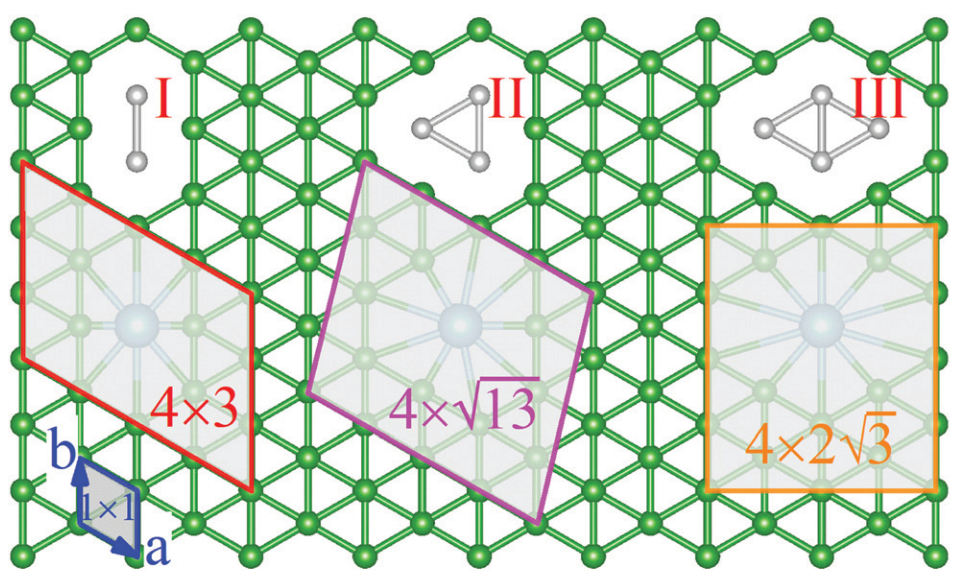
\includegraphics[width=1.0\textwidth]{figs/ch5_how_cell_choose.png}
  \centering
  \caption{单层硼化钛的结构生成示意图。在\rom{1}型、\rom{2}型和\rom{3}型中,一个钛原子分别替代两个、三个和四个硼原子。蓝线勾勒出的菱形表示二维三角晶格的单元格。还同时显示了超胞。大的天蓝色球和小的绿色球分别代表钛原子和硼原子。灰色的球代表要被取代的硼原子。}
  \label{fig:ch5_how_cell_choose}
\end{figure}

\section{单层TiBn的结构多样性与稳定性}
在绪论部分已经介绍了以过渡金属为中心的多配位硼轮平面团簇能够表现出很好的结构稳定性,同时结合了已经有理论预测报导的由过渡金属和硼所构成的稳定二维平面结构。我们因此认为过渡金属和硼能够形成种类多样且拥有新颖优异的物理化学的二维材料。在论文本章节的工作中,我们选择四周期第一系过渡金属钛作为嵌入硼平面的金属原子,探索其可能出现的稳定平面构型。

在该章所描述的工作之前,有如下一些文献预测报导了钛硼二维材料。2014年由Zhang等预测报导的单层\ce{TiB2}结构\cite{zhang2014prediction},结构上,钛原子由六个硼原子包围,硼原子形成蜂窝状结构。该化合物的能带结构中存在狄拉克锥,最大费米速度为\SI{0.57e6}{\meter\per\second},约为石墨烯的一半。
2017年由Qu等所报导的单层平面\ce{TiB4}结构\cite{qu2017two},钛原子由八个硼原子包围组成八配位的钛硼结构,八个硼原子到中心钛原子的距离均相等,且从侧视图可以看到,整个结构是一个完美的平面,原子之间没有起伏。
2017年Wang\cite{wang2017semimetallic}等报导了多种二维钛硼平面构型,构型中的钛硼原子数比从$1:2$到$1:16$,这一系列的构型可分为两大类,一类为钛硼所组成的单层平面结构,一类为钛原子处在两层硼平面之间的三明治结构。其中的\ce{TiB12}的能带结构中存在狄拉克锥,通过对该结构施加横向张力,\ce{TiB12}的功函数和电导能够被调控。

需要强调的是,所有已经报导的钛硼二维结构都是通过材料搜索的方法发现的。
全局材料搜索的方法有其一定优势,它只需要极少的起始变量就能对特定化学配比的化合物在势能面上以很高的自由度进行材料搜索。
但也因为自由度过高,搜索过程中所可能经历的构型数量非常巨大,而其中的许多相近的初始结构往往会在结构优化后变为相同的构型,这在一定程度上即浪费时间,也浪费了计算资源。
另外,固定元素之间形成的化合物往往会存在特定的结构特征,利用先验的引入结构特征将能够确定更合理的设置初始构型集合,从而大大减少计算过程中所需要的时间,减少计算资源的浪费。
以二维钛硼结构为例,我们可以发现,稳定的钛硼构型都是由钛为中心,硼环绕的超多配位结构,这也恰好符合硼与过渡金属形成多配位团簇时出现的结构稳定性。

以此为出发点,我们将所要探索的二维钛硼结构的集合限制在钛硼单层,并且钛原子作为中心原子被硼原子环绕。利用这样的初始结构,我们优化得到了全部已经报导的钛硼单层二维结构,并发现了一些新的具有新颖性质的稳定结构。我们的计算覆盖了很大的化学配比范围,并基本能够确保包含了所有可能的结构组合。同时,所需要计算的构型数量也并不很大,通过与高通量工作流工具结合,能够很快完成结构的优化和性质的计算。

硼原子构成硼平面的结构多样性丰富,但结构的区别均体现在空位分布位置的不同上,也就是说,硼原子网络始终保持为三角格子。过渡金属硼构成的单层平面结构,过渡金属均采取多配位的结构,同时硼网络均能够看做是三角各自轻微程度扭转而成的,如图\ref{fig:ch5_cell_change}所示,我们展示了如何从初始构型结构优化过程中通过胞和原子的轻微位置变化获得新的稳定结构。利用这样的结构上的特征,我们选择在硼原子构成的三角格子网络中用过渡金属原子嵌入网络并替换一个或多个硼原子来构造初始平面单层钛硼网络。这样在结构优化过程中,原子仅仅在原始位置周围移动调整网络的空间结构,即保证能够在势能面的每个可能局域极小值附近都有初始构型,从而对势能面上的所有局域极小结构进行遍历,并考察结构稳定性。

\begin{figure}
  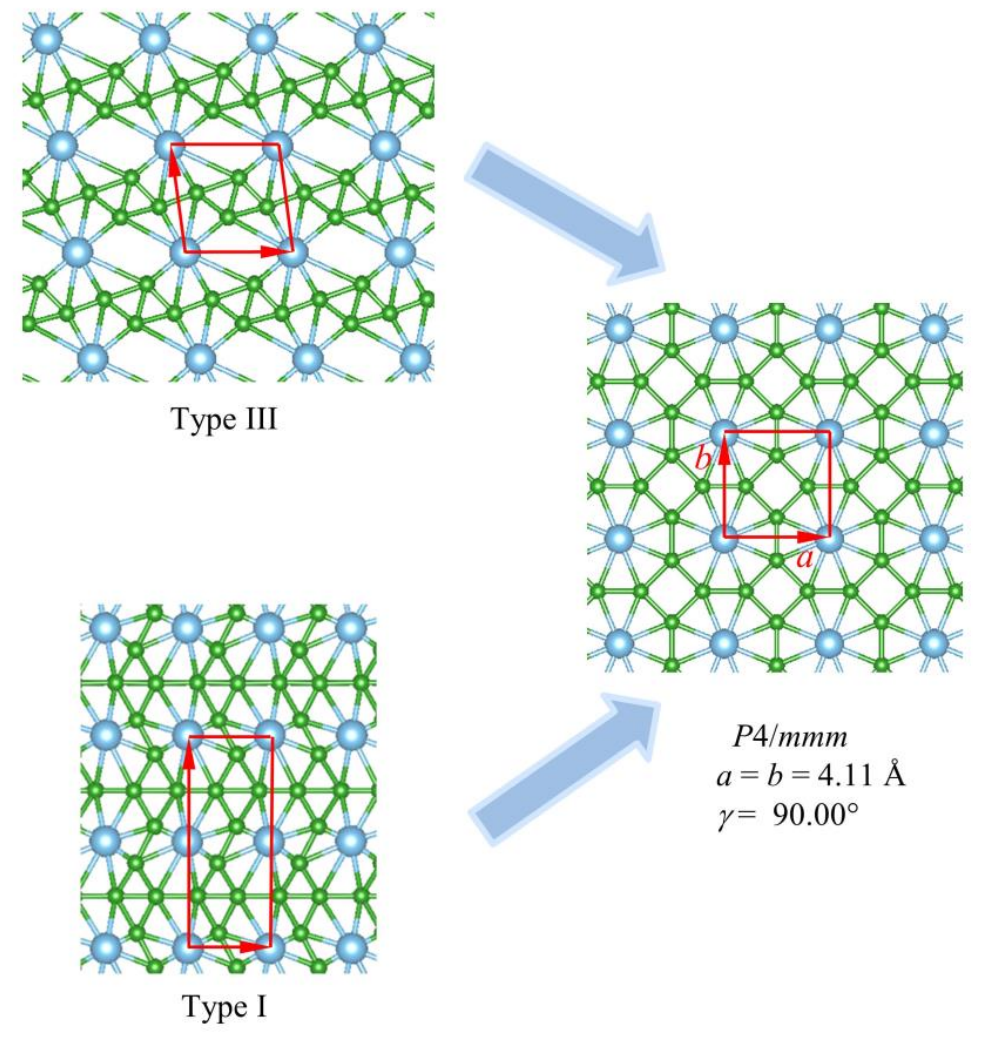
\includegraphics[width=1.0\textwidth]{figs/ch5_cell_change.png}
  \centering
  \caption{分别从\rom{1}型和\rom{3}型的初始构型演变为最后稳定的\ce{TiB4}结构}
  \label{fig:ch5_cell_change}
\end{figure}

下面小节将详细描述初始结构的生成过程,与其结构稳定性的考察过程。

\subsection{结构多样性与结构的生成}

之前文献报导的二维\ce{TiB2}化合物为三明治夹层结构,硼原子形成两层硼平面,钛原子在两层硼平面中间作为插层并与周围的硼原子成键,其中钛原子与硼原子之间的距离为\SI{1.19}{\angstrom}。类似的过渡金属-硼构成的三明治夹层结构在其他的钛硼、铁硼二维结构中也由发现。
而我们的工作,我们将搜索的结构范围限制在单层钛硼结构,旨在探究钛原子与硼形成单层的钛硼平面,并对比所有这类单层平面的结构稳定性。
同样的方法可以很容易地拓展到三明治夹层结构的结构预测中。
为得到这样的单层过渡金属硼平面,我们按照如下的方法来构建初始构型。首先,确保硼原子按照三角格子密堆的形式形成硼单层网络,其次,在网络中插入过渡金属钛原子与硼成键。
然而,由于过渡金属的半径较硼的大的多,其原子很难只是通过替换单个硼原子,来与硼原子网络中的其余硼原子通过六配位的方式来嵌入硼原子网络中而形成二维钛-硼单层结构。
根据过渡金属与硼形成轮状团簇时实验观测到的都是多配位的团簇这一结论,我们认为,在单层过渡金属-硼平面中,过渡金属同样应该倾向于与硼原子形成大于六的高配位。因此,综上两个原则,我们选择初始结构应为在三角硼平面网格的基础上,通过过渡金属替换多于一个的相邻的硼原子来构建结构。所构建的一系列初始构型的多样性可以从以下两点体现:
\begin{itemize}
  \item 可以将硼原子构成的网格以不同的胞进行划分,这里不等价胞的选取我们用到了第\ref{chapter:unique}章所介绍的查重算法,并在我们自己编写的代码上实现。
  \item 相邻的多个硼原子可以有多种聚集方式,而且可以出现在给定单胞的不同的位置。
\end{itemize}
但由于晶格的对称性,所生成的许多结构事实上是互相等价的,在这里等价结构的查重我们用到了第\ref{chapter:unique}章中的固定胞不同结构的查重算法,同样在我们自己编写的软件中实现。下面将针对钛硼单层的初始结构,具体描述这两类体现多样性的查重算法是如何实现的。

首先,我们通过对硼平面的原胞(图\ref{fig:ch5_how_cell_choose}中左下角的深蓝色$1\times 1$晶胞)按不同方式进行展开,得到更大的硼三角超晶格单胞。我们使用厄米标准型矩阵(HNF)\cite{hart2008algorithm}来展开不重复的超胞。这里,我们限定所要考察的结构的尺寸,最大不超过\num{16}倍的原胞面积,即厄米标准型矩阵的行列式的值最大不超过\num{16},因为原胞中仅有一个硼原子,所以其行列式的值也是元胞中的硼原子数量,我们最大得到的硼原子超胞就包含\num{16}个硼原子。每种厄米矩阵对应一种超胞形式,不同的厄米矩阵可以有相等的行列式值,相同的行列式的厄米矩阵代表原子数相同但超胞不等价的两种超胞构型。图\ref{fig:ch5_how_cell_choose}展示了三种不同面积的超胞。在获取固定的超胞后,我们对硼原子进行替换,用一个过渡金属原子一次性替换两个三个或四个硼原子,将过渡金属放在所替换的硼原子的空位的中心。
如图\ref{fig:ch5_how_cell_choose}所示阴影部分中的替代,共有三种方式,分别对应替换两个,三个和四个硼原子,分别形成过渡金属与相邻硼原子配位数为八,九和十的三种结构形式,我们将其初始结构分别命名为\rom{1}型\rom{2}型和\rom{3}型初始构型。替换后的构型会存在等价的构型,我们通过查重算法将等价的构型去除。同时需要提到的是,根据已知经验,过渡金属应该与硼形成配位,而金属-金属直接相连的结构能量上并不占优,为验证这个条件,我们在其中一个超胞下面的构型中,测试了几个金属金属相连的生成构型,结果显示与相同化学计量的构型相比,其能量高出许多。

最后,通过以上步骤,我们一共获得了胞面积小于等于16的超胞下取代后的构型,\rom{1}型\num{210}个,\rom{2}型\num{98}个,\rom{3}型\num{150}个。这样的数量与全局搜索算法所需要的总数相比少了许多(全局搜索算法对特定原子数配比,需要进行上千个结构的优化计算)。值得关注的是,我们使用较少的计算量就能够发现各种{\textbf{不同配比下}}的全局搜索所能发现的全部单层稳定构型,并还发现了能量比已经报导的更低的构型,这个结果我们将在下一节详细叙述。这种搜索策略高效的原因,是因为我们在初始结构的生成中较好的应用了已知的结构上的样式特征,即硼三角网格的过渡金属硼形成多配位。

\begin{figure}
  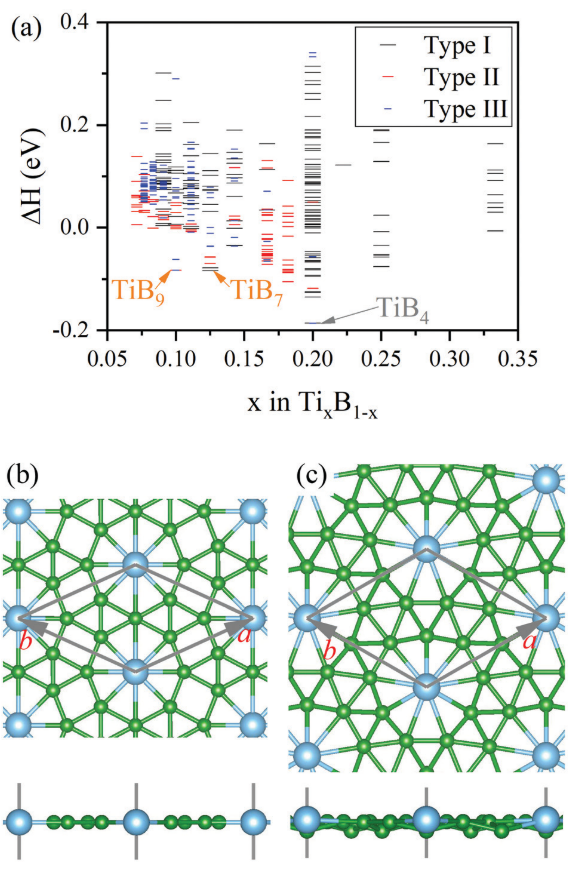
\includegraphics[width=0.72\textwidth]{figs/ch5_energy_hull.png}
  \centering
  \caption{(a)单层硼化钛的形成焓随钛浓度的变化。预测的(b) \ce{TiB7}和(c) \ce{TiB9}的原子结构的俯视图和侧视图。}
  \label{fig:ch5_energy_hull}
\end{figure}

对上面提到的生成的钛硼原子比例从$1:2$到$1:13$的各种钛硼单层构型,在进行结构优化后,我们还对其进行了能量和电子结构的高通量计算,并对每种钛硼原子比例下能量较低的构型分析了其超导性质。

\subsection{单层钛硼结构的稳定性}

由于钛-硼键的键长和硼-硼键的键长之间存在巨大的差别,我们认为钛硼不容易出现六配位的结构,比如在过往报导的文献中,\ce{TiB4}单层是一个全平的平面,其中钛和硼形成八配位的等边多边形,以及硼硼之间形成的四边形,如图\ref{fig:ch5_cell_change}右边的结构优化后的\ce{TiB4}所示。因此我们认为该结构是有一个钛原子处于中心的\ce{Ti}@\ce{B8}轮状团簇图案平铺而成的。

如上一节所述,如图\ref{fig:ch5_how_cell_choose}所示,我们在硼三角网格平面引入多空位(\rom{1}型,\rom{2}型和\rom{3}型分别代表替换两个三个和四个相互连接的硼原子),并在大空位中心放入过渡金属钛原子形成八元九元和十元环的钛硼结构。并基于HNF矩阵和结构识别,我们生成了钛硼单层结构的初始构型并对他们进行了结构优化和能量的计算。为了描述钛硼单层的稳定性和钛原子在结构中占比的关系,我们定义下列形式的单层构型形成能:
\begin{equation}
  \Delta H = E_{Ti_xB_{1-x}} - xE_{Ti} - (1-x)E_{B},
\end{equation}
其中$E_{Ti_xB_{1-x}}$、$E_{Ti}$和$E_B$分别是对应钛硼构型单胞、体相六方密堆钛和稳定$\alpha$-硼的总能量,钛原子在其稳定的六方密堆体相结构中的原子能量,以及单个硼原子在硼平面中的能量。

图\ref{fig:ch5_energy_hull}(a)展示了各个\ce{Ti_xB_{1-x}}构型的形成能$\Delta H$随着钛原子在结构中占比的变化。值得注意的是,其中\ce{TiB4},即已经被报导的平面钛硼单层结构有着最低的形成能,该构型可以分别由如图\ref{fig:ch5_cell_change}左边两个分别属于\rom{1}型和\rom{3}型的初始结构得到。在钛的比例大于\num{0.2}时,初始结构主要是\rom{3}型,因为此时需要在超胞中去除更多的硼原子来放入一个钛原子。而需要代替较少的硼原子的\rom{1}型和\rom{2}型结构则更多的是钛比例较少的构型。

在钛硼比为$1:7$的\ce{TiB7}结构中,形成能最低的结构如图\ref{fig:ch5_how_cell_choose}(b)所示,它是一个全平的平面,优化后该结构的晶格参数为:$a=b=\SI{5.72}{\angstrom},\gamma=\SI{130.94}{\degree}$,该结构空间群为$Cmmm$。该结构中,钛原子与硼原子组成八元环,其中的钛硼键的长度分别为\SI{2.15}{\angstrom},\SI{2.18}{\angstrom}和\SI{2.37}{\angstrom}。结构中硼原子之间还组成了三元环与四元环(此处硼硼原子成键的标准选择为化合物中出现的最大的硼-硼原子键作为上限,超过该长度则认为硼硼原子不成键),因此该结构可以认为是由\ce{TiB8}轮状碎片与三元四元硼碎片平铺拼接而成的。
我们同样在图\ref{fig:ch5_tib7_last3}中展示了该钛原子浓度下能量最低的三种构型,以及能够优化到这些结构的初始构型,可以看到,初始结构和最终结构的原子位置只是发生了很小的变动,说明了我们生成的初始构型的方式是合理的。其中能量次低的构型为$P2/m$空间群,每个原子的平均形成能与最稳定构型相差了6meV,这个不大的能量差别说明我们方法对特定构型势能空间局域极小值的判断精度达到了$<$\SI{10}{\meV}的级别,能够区别搜索能量相差不是很大的构型。这个能量次低的构型与最低的构型非常相似,区别是该构型的$a,b$晶格参数不相等,并且这个结构是之前文献\cite{wang2017semimetallic}使用全局搜索软件USPEX得到的该配比下的最稳定构型。能量第三低的结构为$Pm$空间群,能量比次低结构高出了\SI{14}{\meV}。

\begin{figure}
  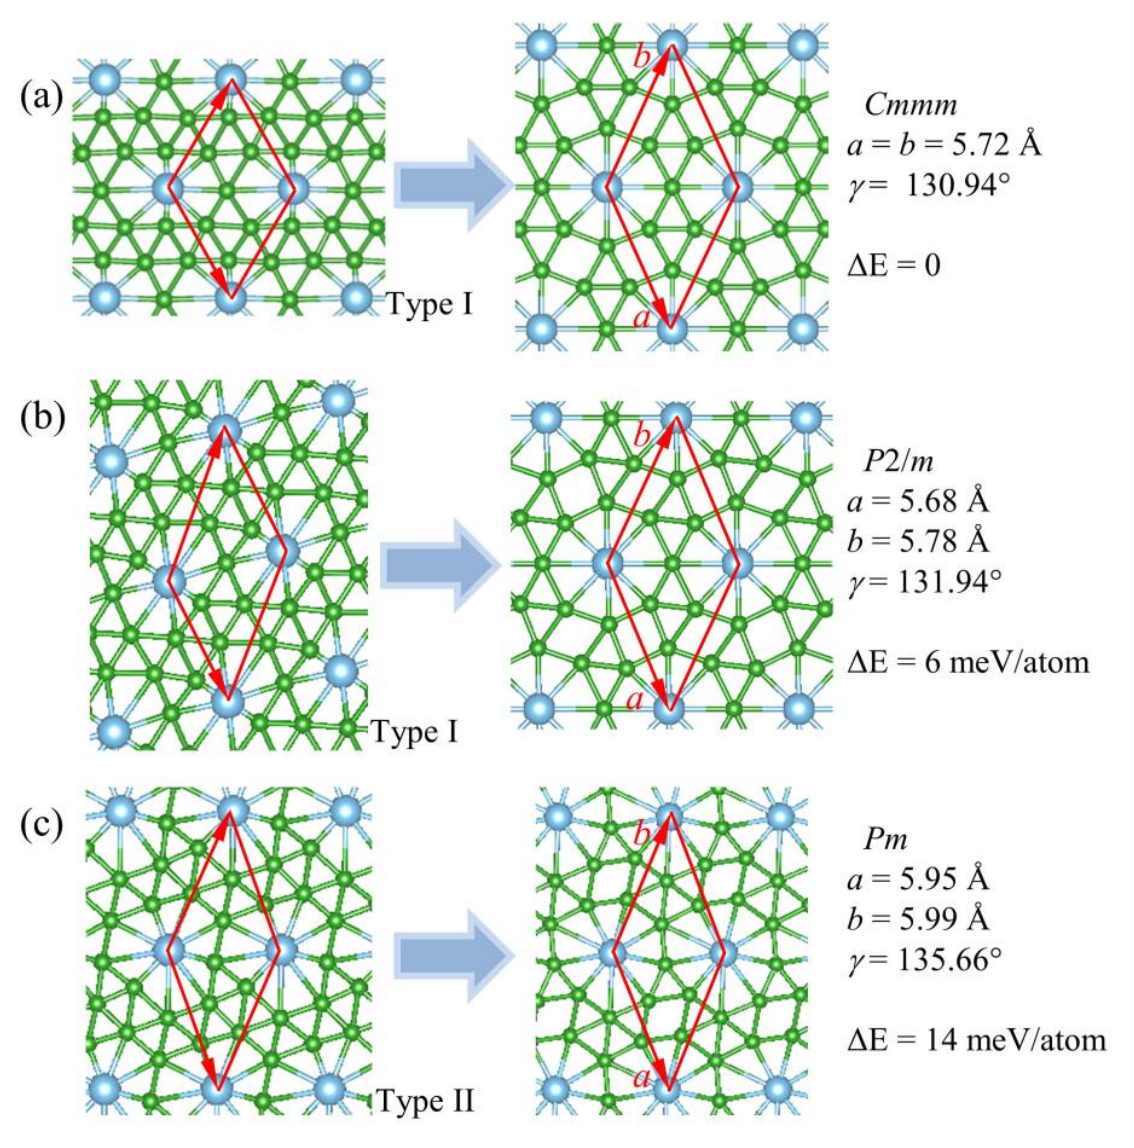
\includegraphics[width=0.72\textwidth]{figs/ch5_tib7_last3.png}
  \centering
  \caption{\ce{TiB7}能量最低的三种构型,以及它们的初始构型。}
  \label{fig:ch5_tib7_last3}
\end{figure}

我们还着重考察了钛硼比例为$1:9$的构型,其能量最低的构型如图\ref{fig:ch5_energy_hull}(b)所示,晶格参数为$a=b=\SI{5.83}{\angstrom},\gamma=\SI{120}{\degree}$,空间群为$P31m$。结构中有两种不等价(不同维科夫位点)的硼原子,每个钛原子被九个硼原子所包围,钛硼键的键长分别为\SI{2.22}{\angstrom}和\SI{2.43}{\angstrom}。硼原子形成三元环并和钛-硼构成的九元轮状碎片相连接。能量最低的构型可以对应由如图\ref{fig:ch5_tib9}所示的\rom{2}型\rom{3}型两种初始构型优化而来。
这个稳定的构型同样已经被之前的文献\cite{wang2017semimetallic}报导,这再次说明了我们所采用的搜索算法的可靠性。

\begin{figure}
  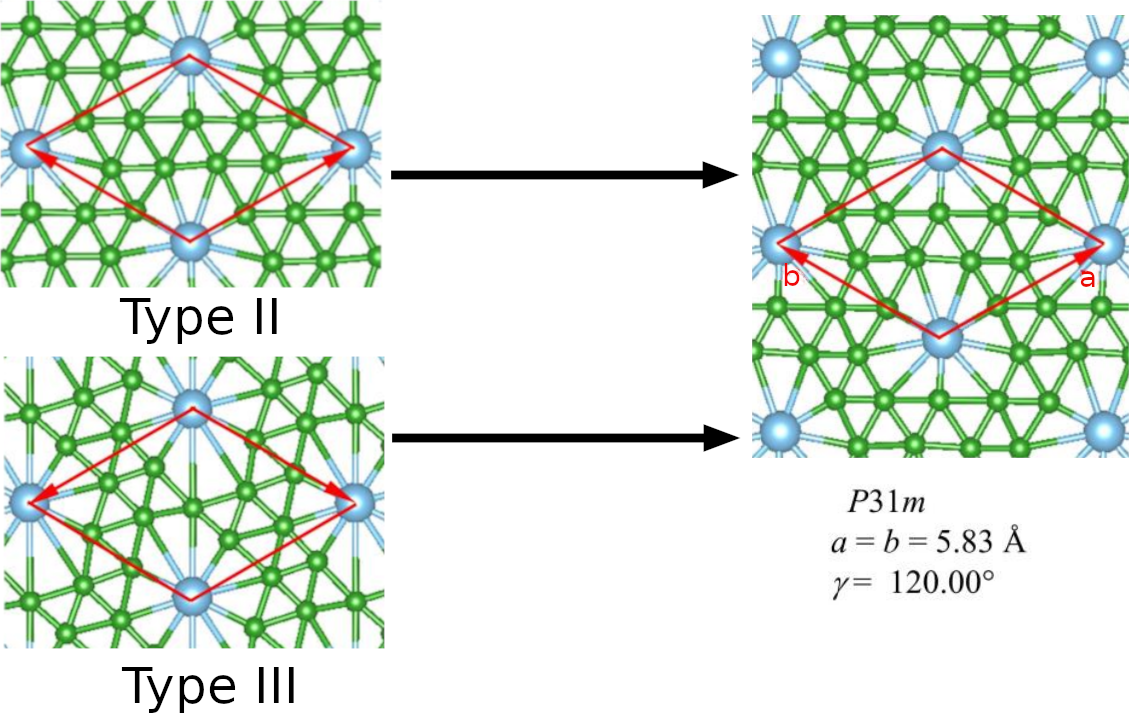
\includegraphics[width=0.82\textwidth]{figs/ch5_tib9.png}
  \centering
  \caption{\ce{TiB9}能量最低的构型,以及初始构型}
  \label{fig:ch5_tib9}
\end{figure}

我们分析了\ce{TiB7}和\ce{TiB9}两个单层平面能带,态密度和投影态密度等电子结构性质如图\ref{fig:ch5_bands}。\ce{TiB7}和\ce{TiB9}均为金属,费米能级穿过其能带。\ce{TiB7}单层费米能级附近的态主要是由钛的$d$轨道和硼的$p$轨道构成的,而在\ce{TiB9}中,费米能级附近的波函数主要来自于钛的$d$轨道。与\ce{TiB4}单层相比,$d$轨道能级在单层中构成了一个接近水平的能带,这个轨道大大增加了费米能级附近的态密度,因此可能使其成为潜在的超导材料。

该研究所涉及的初始结构的钛硼原子比例共\num{14}种,除了上面详细描述的\ce{TiB7}和\ce{TiB9}两种结构,其它浓度下能量最低的构型分别展示在图\ref{fig:ch5_all_configs}中。我们可以发现,钛的浓度过高或过低都不利于结构的稳定,当钛在结构中占比过高时,钛原子倾向于聚集形成团簇,并和硼原子构成的团簇分离。当钛原子浓度过低时,钛原子的表现为扭曲了硼的平面稳定结构,并且,由于我们没有考虑钛原子和空位同时出现的情况,硼的无空位三角网络并不稳定,因此同样难以获得稳定的结构。另外在这些结构中能发现另一有趣的现象,其中\ce{TiB4},\ce{TiB7},\ce{Ti2B9}以及\ce{TiB5}这几个各自浓度下能量最低的构型形成了{\textbf{全平的完美的二维结构}},说明这些浓度下电子在平面上很好的分布。我们尚不知道这种全平的完美二维单层是否由特殊的性质,但为结构的多样性以及结构的研究提供了很好的素材。

\begin{figure}
  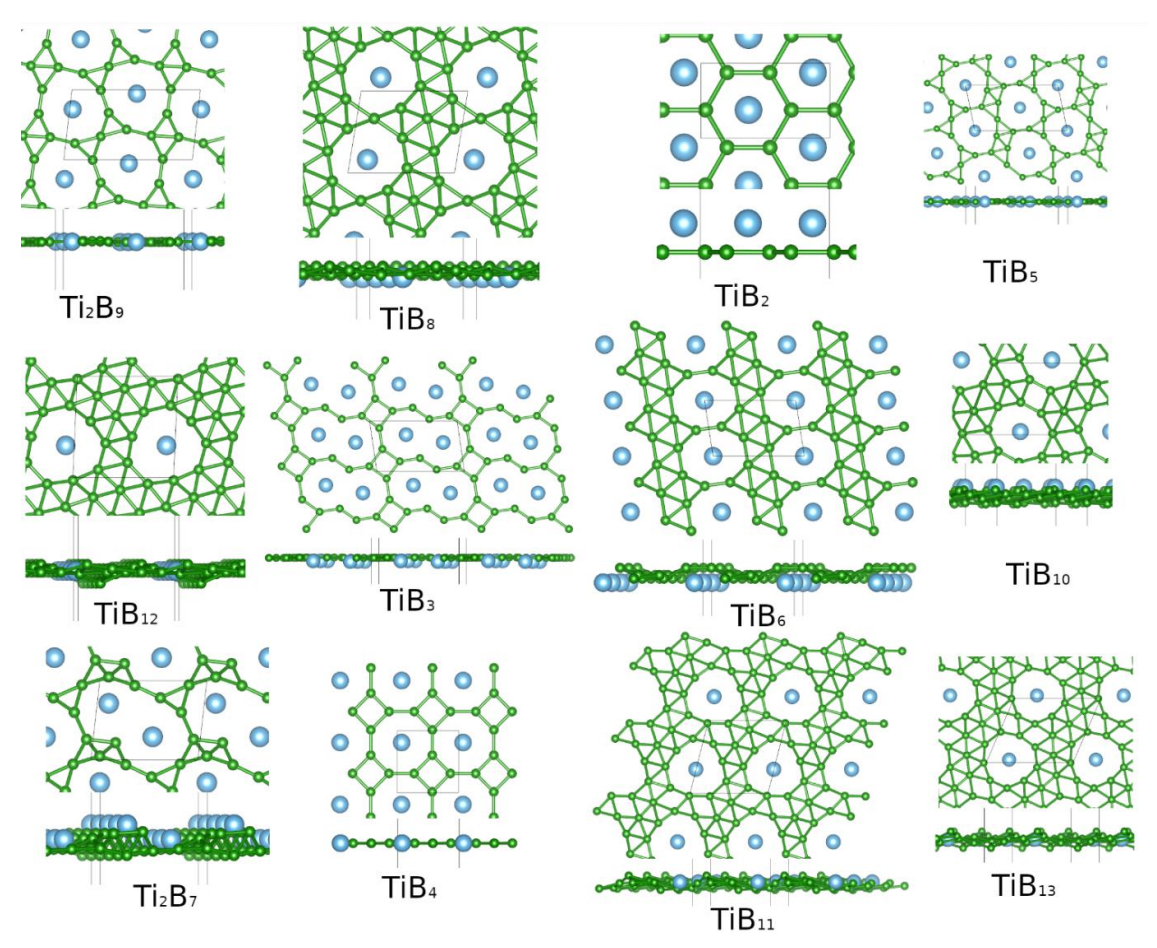
\includegraphics[width=0.96\textwidth]{figs/ch5_all_configs.png}
  \centering
  \caption{钛硼单层在所有我们探索的浓度下能量最低的构型,图片展示了结构的俯视图和侧视图。}
  \label{fig:ch5_all_configs}
\end{figure}

\section{钛硼二维材料的超导性质}
为探究潜在的超导性质,我们分析了\ce{TiB7},\ce{TiB9}单层和\ce{TiB7}双层的电声耦合性质。根据第\ref{chapter:theory}章中的叙述,定义的由Eliashberg谱得到的无量纲的电声耦合常数$\lambda$有以下形式:

\begin{equation}\label{eq:lambda_coupling}
  \lambda = 2 \int d\omega \frac{\alpha^2 F(\omega)}{\omega}.
\end{equation}
其中$\alpha^2 F(\omega)$是Eliashaberg谱函数,可以通过下列形式计算得到,

\begin{equation}\label{eq:elishaberg_calc}
  \alpha^2 F(\omega) = \frac{1}{2\pi N(\epsilon_F)}\frac{1}{N_{\bm{q}}}
  \sum_{\bm{q}j} \frac{\gamma_{\bm{q}j}}{\omega_{\bm{q}j}}
  \delta(\omega-\omega_{\bm{q}j}),
\end{equation}
表达式中$N(\epsilon_F)$是费米能级处的电子密度,公式中的狄拉克$\delta$函数在实际计算中可以用高斯函数近似。$\omega_{\bm{q}j}$和$\gamma_{\bm{q}j}$分别是模为$j$的声子在波矢$\bm{q}$处的频率和线宽。最后表达式中的$N_{\bm{q}}$是第一布里渊区所统计的波矢数量,在实际计算中,为了得到准确的结果,我们往往需要很密的$\bm{q}$点的划分。式中给定波矢和特定声子振动模式下的电声耦合系数为:

\begin{equation}
  \lambda_{\bm{q}j} =
  \frac{\gamma_{\bm{q}j}}{\pi \hbar N(\epsilon_F) \omega^2_{\bm{q}j}},
\end{equation}
使用该等式,体系的各向同性耦合常数$\lambda$可写为以下形式:
\begin{equation}\label{eq:lambda_from_phonon}
  \lambda = \frac{1}{N_{\bm{q}}}\sum_{\bm{q}j} \lambda_{\bm{q}j}.
\end{equation}
从声子谱中计算得到每个振动模式不同频率下的耦合系数后代入上式(\ref{eq:lambda_from_phonon})就能得到无量纲的材料的电声耦合常数。

\begin{figure}
  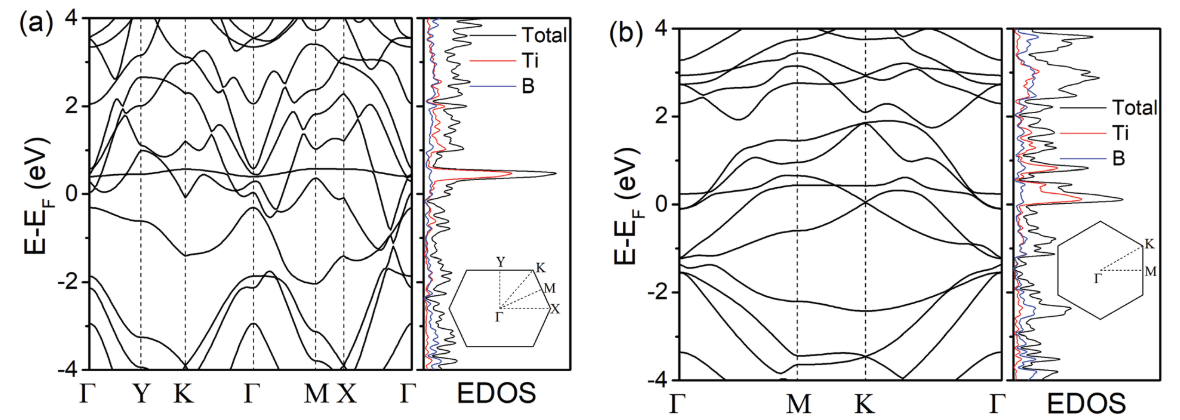
\includegraphics[width=0.96\textwidth]{figs/ch5_bands.png}
  \centering
  \caption{\ce(TiB7)和\ce{TiB9}的能带和态密度。}
  \label{fig:ch5_bands}
\end{figure}

\subsection{单层\ce{TiB7}的超导性质}
图\ref{fig:ch5_tib7_sc_all}展示了\ce{TiB7}单层的声子谱及各个振动模式不同频率的声子线宽$\gamma_{\bm{q}j}$,Eliashhberg函数$\alpha^2 F(\omega)$和$\lambda(\omega)$ ($\omega$为计算的声子的频率上限)。首先可以确定的是,结构可以在单层状态稳定存在,因从图\ref{fig:ch5_tib7_sc_all}(a)的\ce{TiB7}声子谱中没有虚频。
从图中可以看出,主要是低频($<$\SI{400}{\per\cm})的振动模式贡献了电声耦合。
从Eliashberg函数$\alpha^2 F(\omega)$可看出,在频率为约\SI{200}{\per\cm}处有数个尖峰,其主要是由该频率位于$\Gamma$点周围的声子贡献的,此处在$\Gamma$点的声子线宽较大。我们将$\Gamma$点附近频率从\SI{160}{\per\cm}到\SI{240}{\per\cm}处的声子谱放大在图\ref{fig:ch5_tib7_sc_all}中展示,
此处有四种振动模式$\omega_1$、$\omega_2$、$\omega_3$和$\omega_4$,
分别代表了如图\ref{fig:ch5_tib7_sc_all}(b)所示的四种振动。
其中,$\omega_1$为面内的剪切模(图\ref{fig:ch5_tib7_sc_all}(c)),它的振动模式的对称性为$C_3$。图\ref{fig:ch5_tib7_sc_all}(d)(e)(f)为其余三个垂直于面平面的振动模式,通常在文献中,将这种垂直于面的振动模式称为呼吸模。在四种模式中,剪切模$\omega_1$和呼吸模$\omega_3$、$\omega_4$的声子线宽较大。$\omega_2$处的声子线宽较小,但由于其该带很平,在态密度中这一频率处贡献很大。综上两个因素导致了在\SI{200}{\per\cm}附近Eliashberg函数的绝对值较大,贡献了很大的电声耦合。
根据McMillan-Allen-Dynes参数化Eliashberg方程,我们可以估计超导临界温度$T_c$:
\begin{equation}
  T_c = \frac{\omega_{\mathrm{log}}}{1.2}
  \exp{\left[ {-\frac{1.04(1+\lambda)}{\lambda-\mu^*(1+0.62\lambda)}} \right]}
\end{equation}
其中$\omega_{\mathrm{log}}$为Eliashberg函数在全频率范围的对数平均,表示如下:
\begin{equation}
  \omega_\mathrm{log} = \exp \left[ {\int d\omega \log(\omega)W(\omega)} \right],
\end{equation}
其中的权重$W$定义为:
\begin{equation}
  W(\omega) = \frac{2}{\lambda} \frac{\alpha^2 F(\omega)}{\omega}.
\end{equation}

\begin{figure}
  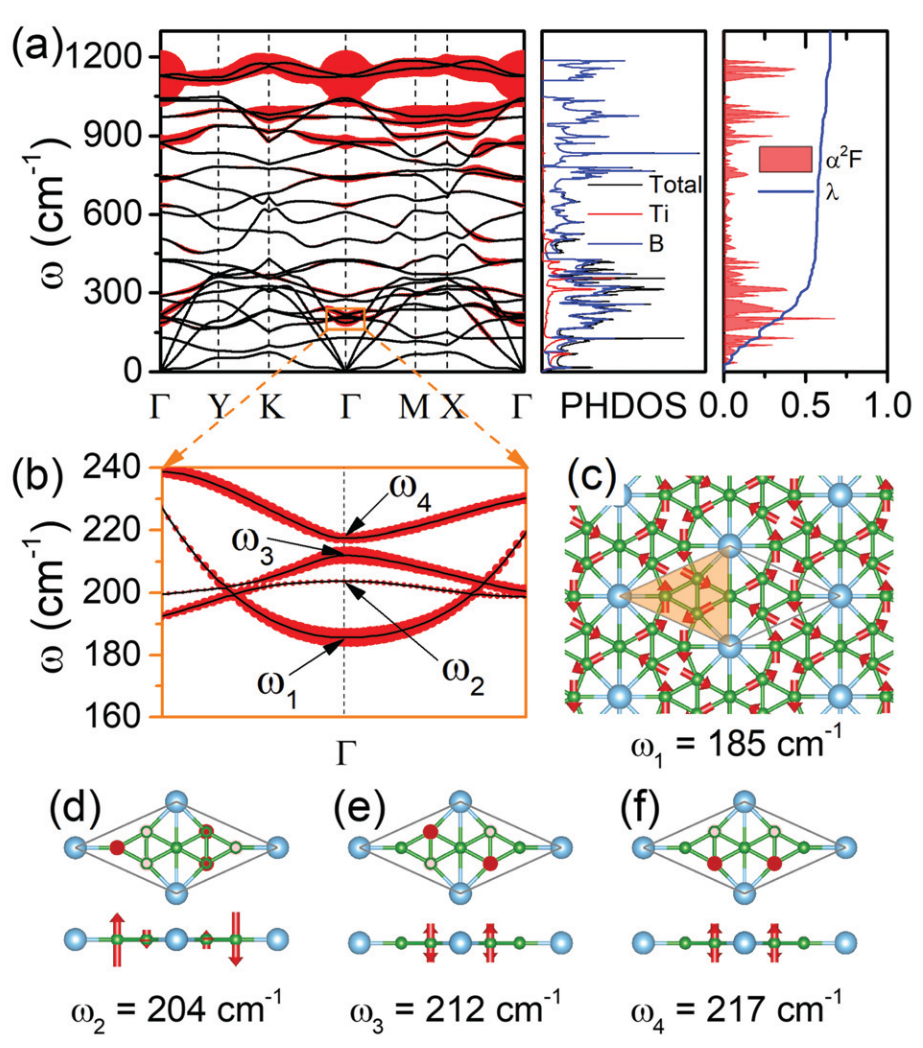
\includegraphics[width=0.96\textwidth]{figs/ch5_tib7_sc_all.png}
  \centering
  \caption{(a)红色包围的区域中声子色散与声子线宽$\gamma_{qj}$、声子态密度以及单层\ce{TiB7}的Eliashberg函数$\alpha^2 F(\omega)$和$\lambda(\omega)$。(d-f)层的呼吸模。红色箭头及其长度代表了相应振动模式的方向和振幅。}
  \label{fig:ch5_tib7_sc_all}
\end{figure}

根据之前关于硼材料研究的文献\cite{penev2016can,zhao2016superconductivity,zhao2018multigap,liao2017phonon,yan2020superconductivity},
上面经验公式中的库伦排斥势$\mu^*$我们选取了$\mu^*=0.1$来计算超导转变温度。图\ref{fig:ch5_tib7_coupling}中展示了电声耦合系数$\lambda_{\bm{q}j}$在倒空间中的变化情况,我们可以看到,在$\Gamma$点附近是一个以$\Gamma$点为中心的哑铃形状的分布,其最大的$\lambda_{\bm{q}j}$值大于\num{1.0}。全部倒空间中的电声耦合系数除了$Y$对称点处均大于\num{0.6}。因而总的电声耦合常数$\lambda$为\num{0.65}。
将$\lambda$代入以上公式中我们得到单层\ce{TiB7}平面的超导转变温度为\num{8.3}K。该超导温度高于报导的锂沉积石墨烯的超导转变温度,即理论计算的超导温度为$T_c=8.1K$\cite{profeta2012phonon},实验测量得到的超导转变温度为\num{5.9}K\cite{ludbrook2015evidence}。
在钛硼化合物中,原子质量较小的硼元素是常规BCS超导电声耦合的主要原因。同样的所有的单层金属硼平面均显示出超导性质,而超导转变温度和硼平面的空位浓度之间存在先减少后增加的关系。当空位浓度为\num{1/9}时,最稳定的$\alpha$-硼平面的超导转变温度为\SI{3.7}{\kelvin}。
当空位浓度增加到\num{1/8}时超导转变温度提高到\SI{5.8}{\kelvin}。我们可以看到,通过引入钛原子增加里材料的电声耦合并提高了超导转变温度$T_c$。
钛单质块体中测量得到的超导转变温度最大为\SI{0.38}{\kelvin}\cite{matthias1963superconductivity},因此在\ce{TiB7}中超导主要是由硼元素所贡献的。

\begin{figure}
  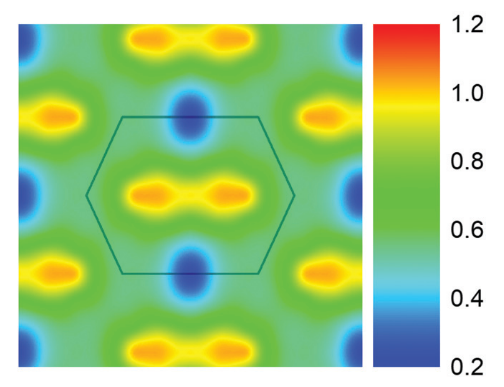
\includegraphics[width=0.72\textwidth]{figs/ch5_tib7_coupling.png}
  \centering
  \caption{电声耦合系数$\lambda_{\bm{q}j}$在倒空间中的变化情况}
  \label{fig:ch5_tib7_coupling}
\end{figure}

二维BCS型超导体\ce{AlB6}中报导了通过拉伸材料可以提高,\SI{12}{\percent}的拉伸应变可以将超导温度提高到30K。我们同样对\ce{TiB7}平面作了相似的拉伸应变,从图\ref{fig:ch5_tib7_strain}中可以看到,拉伸并没有提高超导温度,在施加\SI{5}{\percent}的拉伸应变后材料的超导转变温度降低到了约2K。尽管随着应力的增加$\omega_\mathrm{log}$持续增加,但是总的电声耦合常数和超导转变温度均减小。其中,$\Gamma$点处低频的声子频率随应力增加而增加,高频的声子频率岁应力的增加而减少。图\ref{fig:ch5_tib7_strain}中展示了高频声子和低频声子频率随拉伸应变的变化关系。
我们还在图\ref{fig:ch5_details_strains}中展示了声子谱以及Eliashberg函数随应力变化的详细关系。若拉伸应变会减小超导转变温度,则相反的压缩应变应该增加超导转变温度,如\ce{B5}硼平面\cite{cheng2017suppressed},二维\ce{TiS2}\cite{liao2020doping},
甚至并非属于BCS超导的\ce{FeS}层状结构\cite{nie2009suppression}。然而,对于\ce{TiB7}单层压缩应变在达到\SI{1}{\percent}后结构声子谱中就出现了如图\ref{fig:ch5_tib9_phonon_a}中的严重的虚频,我们认为该强度的应变就会使结构出现相变而丧失超导性质。

\begin{figure}
  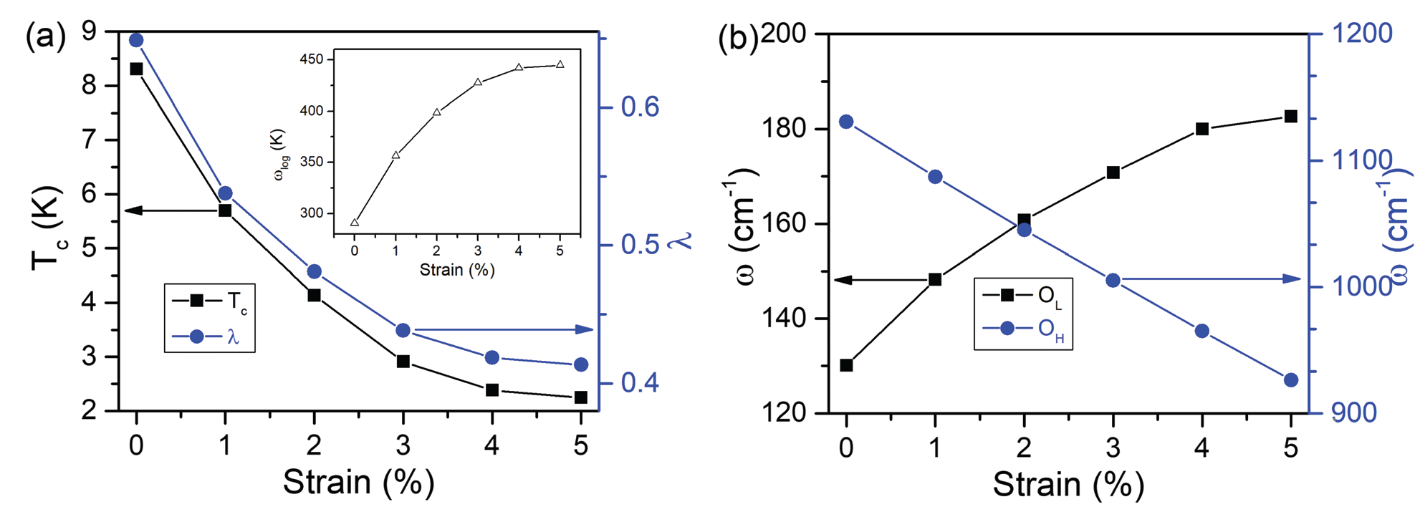
\includegraphics[width=0.96\textwidth]{figs/ch5_tib7_strain.png}
  \centering
  \caption{计算了\ce{TiB7}单层的$T_c$和电声耦合常数$\lambda$随等双轴拉伸应变的变化。以及对数平均声子频率($\omega_{\mathrm{log}}$)的变化。(b)在$\Gamma$处的光学声子的最低($O_L$)和最高($O_H$)频率随应变变化的函数。}
  \label{fig:ch5_tib7_strain}
\end{figure}

\begin{figure}
  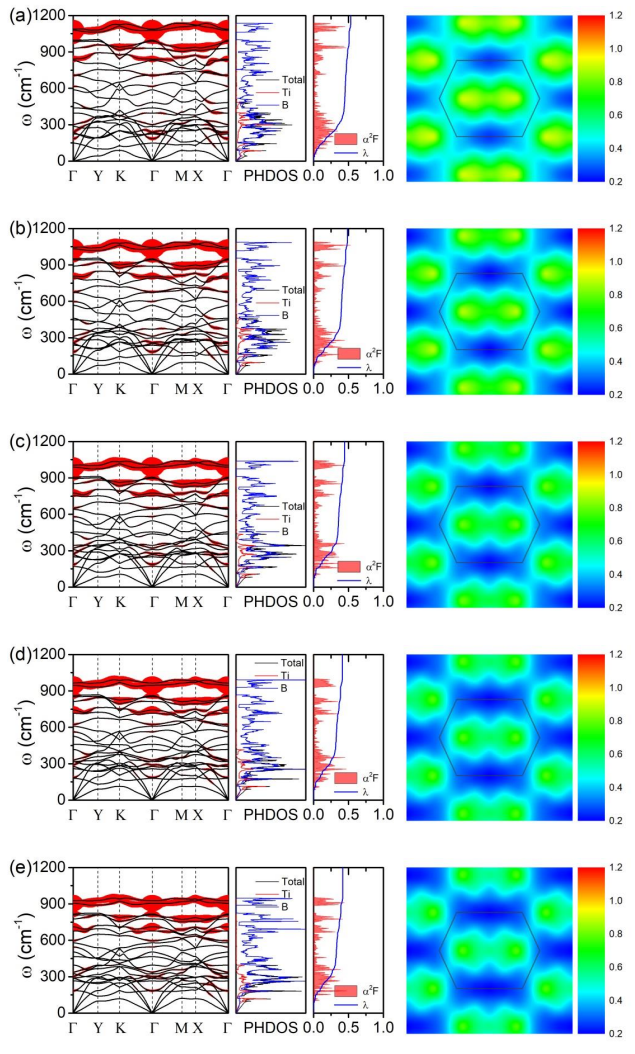
\includegraphics[width=0.88\textwidth]{figs/ch5_details_strains.png}
  \centering
  \caption{在拉伸应变为(a) \SI{1}{\percent}, (b) \SI{2}{\percent}, (c) \SI{3}{\percent}, (d) \SI{4}{\percent}, (e) \SI{5}{\percent},\ce{TiB7}单层薄膜的声子色散以声子线宽$\gamma_{qj}$、声子态密度、Eliashberg函数$\alpha^2 F(\omega)$和$\lambda(\omega)$和耦合常数强度在倒空间的分布。}
  \label{fig:ch5_details_strains}
\end{figure}

作为对比,我们还计算了\ce{TiB9}单层的超导相关性质。如图\ref{fig:ch5_tib9_phonon},该结构声子谱中同样不存在虚频说明其能够以二维的形式稳定存在。电声耦合的计算结果如图\ref{fig:ch5_tib9_phonon}所示,其各向同性平均电声耦合系数$\lambda$为0.40。在$\Gamma$点附近其电声耦合系数最大为$\lambda_{\bm{q}j}$约为0.7.由此可以估计其超导转变温度为\SI{1.2}{\kelvin}。如前面描述的,\ce{TiB7}单层是完全平面的结构,而\ce{TiB9}不同其垂直方向有原子的起伏。
为了研究垂直方向的起伏对超导性质的影响,我们构造了完全平整的\ce{TiB9}构型作为对比,并研究了其声子部分振动模式信息的变化作为参照,以确定是否完全平整的平面能够提高电声耦合从而提高超导性质。
优化后的\ce{TiB9}平面构型的晶格参数增加了\SI{1.2}{\percent},且总能上升了\SI{0.19}{\eV}。然而,计算结果显示该构型有明显的虚频如图\ref{fig:ch5_tib9_phonon_a}所示,因此无法进一步研究电声耦合性质以作为对比。

\begin{figure}
  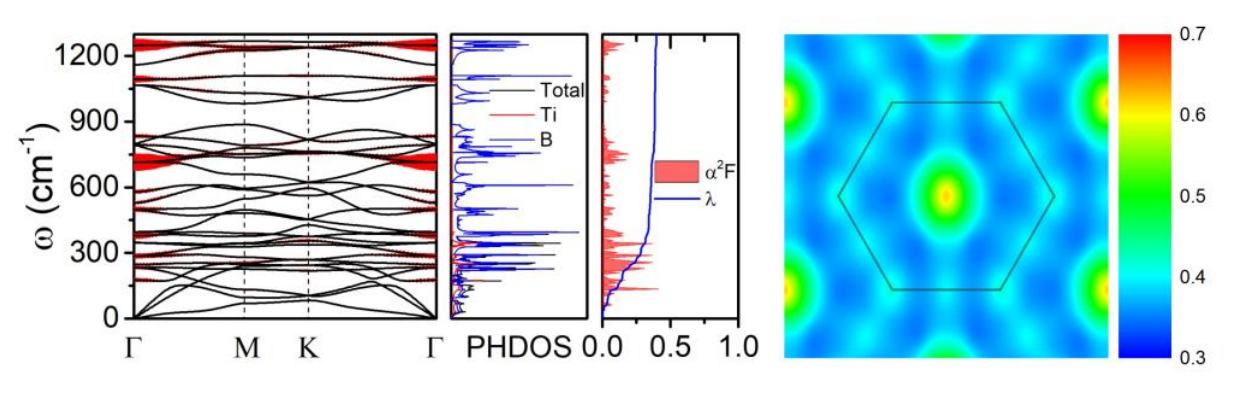
\includegraphics[width=0.96\textwidth]{figs/ch5_tib9_phonon.png}
  \centering
  \caption{\ce{TiB9}单层薄膜的声子色散以声子线宽$\gamma_{qj}$、声子态密度、Eliashberg函数$\alpha^2 F(\omega)$和$\lambda(\omega)$和耦合常数强度在倒空间的分布。}
  \label{fig:ch5_tib9_phonon}
\end{figure}

\begin{figure}
  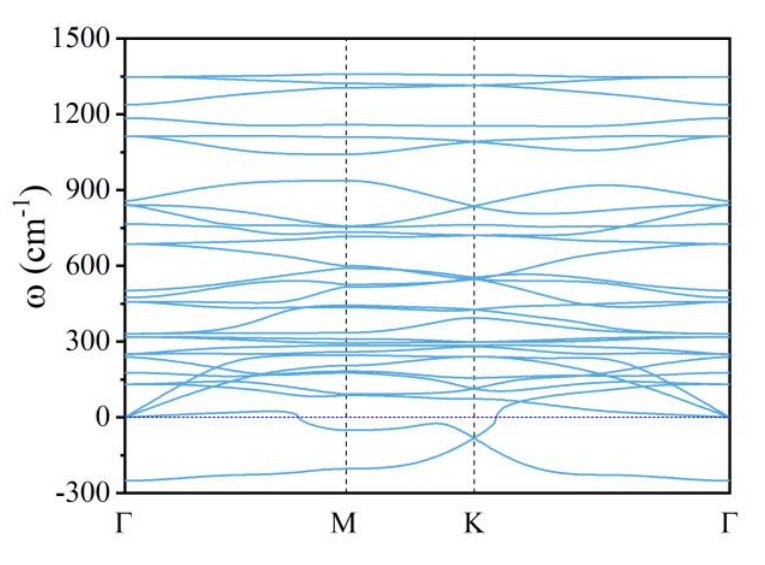
\includegraphics[width=0.72\textwidth]{figs/ch5_tib9_phonon_a.png}
  \centering
  \caption{全平的\ce{TiB9}的声子谱。}
  \label{fig:ch5_tib9_phonon_a}
\end{figure}

\subsection{双层\ce{TiB7}的超导性质}
因为之前报导的有超导性质的过渡金属硼二维材料都是多层的构型,我们考虑通过将\ce{TiB7}堆积为双层构型是否能够提高其超导性质。如下图\ref{fig:ch5_stack_tib7},展示了\ce{TiB7}单层堆叠后形成的双层的声子谱及声子线宽$\gamma_{\bm{q}j}$,Eliashhberg函数$\alpha^2 F(\omega)$和$\lambda(\omega)$。可以确定的是,从图\ref{fig:ch5_stack_tib7}的AB形式堆叠的\ce{TiB7}双层的声子谱可以看出,声子谱中没有虚频说明结构可以在叠层状态稳定存在。
但相比于单层堆叠的\ce{TiB7}构型,双层的\ce{TiB7}费米能级处的电子密度$N(\epsilon_F)$下降了近\SI{25}{\percent}(如图\ref{fig:ch5_stack_tib7}),因此导致电声耦合系数$\lambda$下降了约\SI{22}{\percent},超导转变温度下降了\SI{34}{\percent}。

从图中可以看出,在该双层构型中,同样是是低频($<$\SI{400}{\per\cm})的振动模式贡献了主要的电声耦合。
与单层\ce{TiB7}超导性质计算时相同,经验公式中的库伦排斥势$\mu^*$我们依然选取使用了$\mu^*=0.1$来计算超导转变温度。
根据McMillan-Allen-Dynes方程,我们可以估计超导临界温度$T_c$为\SI{5.5}{\kelvin}。

\begin{figure}
  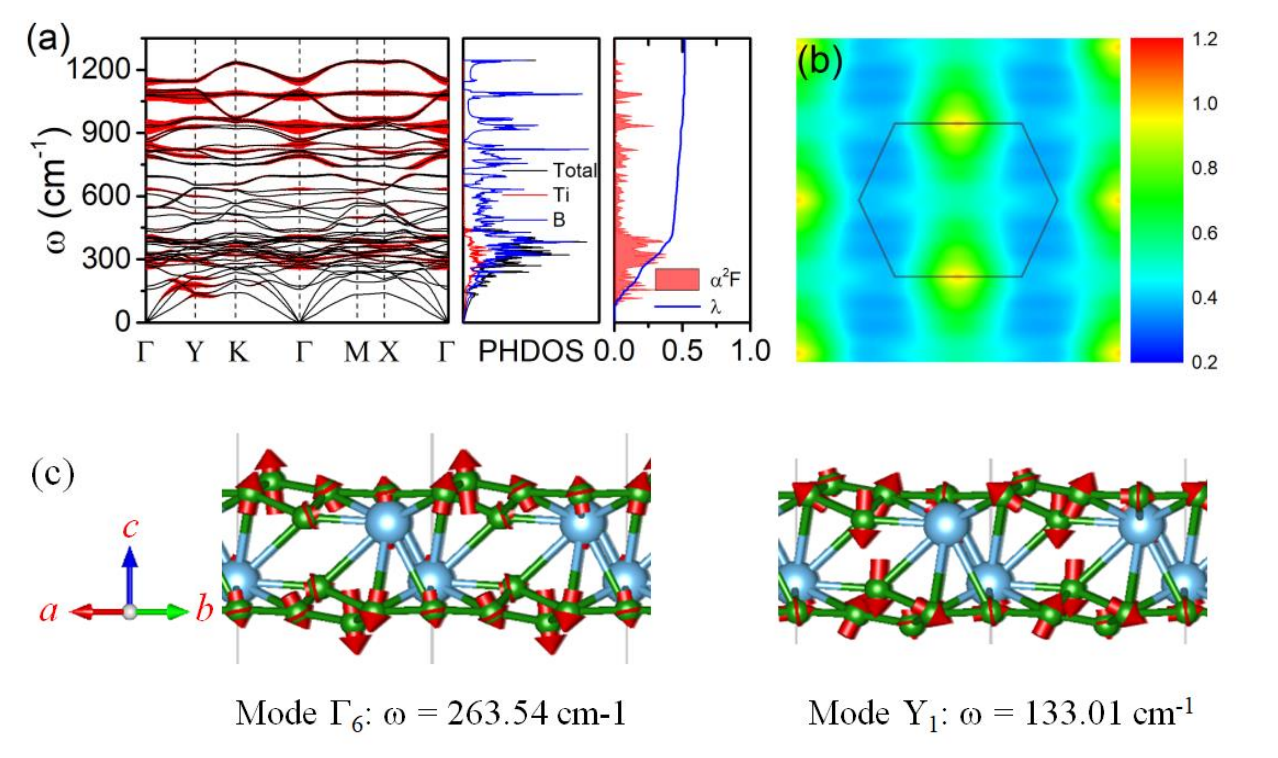
\includegraphics[width=0.96\textwidth]{figs/ch5_stack_tib7.png}
  \centering
  \caption{(a)(b)AB方式堆叠的\ce{TiB7}单层薄膜的声子色散以声子线宽$\gamma_{qj}$、声子态密度、Eliashberg函数$\alpha^2 F(\omega)$和$\lambda(\omega)$和耦合常数强度在倒空间的分布。(c)振动模式$\Gamma_6$和$Y_1$的具体形式。}
  \label{fig:ch5_stack_tib7}
\end{figure}

图\ref{fig:ch5_stack_tib7}中展示了电声耦合系数$\lambda_{\bm{q}}$在到空间中的变化情况,我们可以看到,声子线宽在$Y$对称点附近为最大,这是与单层\ce{TiB7}所不同的,且该处的电声耦合系数为最大值$\lambda_{\bm{q}}\approx 1$。从振动模式中可以看出,在堆叠后双层\ce{TiB7}中每个单层都不再是全平的平面结构,而有原子的起伏,这使得原先单层中对电声有较大贡献的面内的旋转振动模式不再出现。与单层\ce{TiB7}相同,双层\ce{TiB7}的电声耦合同样主要来源于原子质量较轻的硼原子。
我们将本文所研究的和已经报导的钛硼结构的电声耦合和超导性质总结在表\ref{table:sc_all}中。

\begin{table}
  \centering
  \begin{tabular}{lllll}
    \hline\hline
    compounds & $N(\epsilon_F)$ & $\omega_\mathrm{log}$ & $\lambda$ & $T_c$(\si{\kelvin}) \\
    \hline
    \ce{TiB7}单层 & 1.78 & 290.47 & 0.65 & 8.3 \\
    \ce{TiB7}双层 & 1.32 & 409.90 & 0.51 & 5.5 \\
    \ce{TiB9}单层 & 2.25 & 325.97 & 0.40 & 1.2 \\
    \ce{TiB4}单层 & 1.21 & 484.87 & 0.18 & 0.0 \\
    \ce{Ti2B2}单层 & 7.96 & 326.75 & 0.27 & 0.0 \\
    \hline
  \end{tabular}
  \caption{各种二维钛硼结构的超导性质}\label{table:sc_all}
\end{table}
